\subsection{Object-Oriented Imitation Learning}
\label{sec:ooil}
All the methods discussed in Section \ref{sec:lfd} share a common characteristic: they are end-to-end systems that take high-level inputs, such as images, and directly generate the corresponding actions as output. While this approach may work well in simple scenarios, where the scene lacks distracting objects or where such objects are easily identified by the system as being consistently uninvolved in the manipulation, it may struggle in more complex environments. Specifically, it can encounter difficulties when the robot workspace contains objects that are similar to each other, especially if these objects are involved in manipulation for some task variations.

Based on this consideration, this paragraph will describe methods that leverage object priors. This means that the control policy is informed not only by the embedding of the agent scene, which is obtained from a deep architecture, but also by object-level information, such as the bounding boxes of objects in the scene, obtained from an object detector.

The concept of leveraging object priors has been explored in both earlier works \cite{devin2018deep,park2021object} and more recent approaches \cite{belkhale2023plato,zhu2023viola,zhu2023learning,jiang2023vima}.

One of the preliminary works on leveraging object priors was presented by the authors of \cite{devin2018deep}. This work primarily focuses on the challenge of generalization in LfD systems that use an end-to-end approach. In such systems, a task-specific model is trained to predict actions based on raw visual observations. The authors found that while it is possible to achieve good \textit{instance-level generalization}, meaning the model can solve tasks with varying initial configurations using a limited number of samples, achieving \textit{category-level generalization} is more challenging. Category-level generalization refers to the model ability to solve tasks involving different objects. To achieve this, the dataset must include many trajectories involving a wide variety of objects. For instance, if the task is to pour the contents of a bottle into a cup, the dataset should contain trajectories with different types of cups and bottles. However, constructing such a dataset is time-consuming and costly. Moreover, the potential of well-known large datasets in classical computer vision tasks, such as object detection, is not fully utilized.

To address this issue, the authors proposed a paradigm shift by introducing a robotic vision framework that operates on sets of objects rather than raw pixel data. This framework leverages prior datasets to learn a generic object detection model, thereby enhancing category-level generalization without requiring an extensive and diverse dataset. The framework is illustrated in Figure \ref{fig:object_prior_framework} and is composed of several stages:
\begin{itemize}
    \item \textbf{Meta-Attention}. This is a Region Proposal Network (RPN) \cite{fastrcnn}, trained on the well known MSCOCO \cite{lin2014microsoft} dataset. The RPN generates objects proposals, i.e., region of the image that possibly contain an object.
    \item \textbf{Task-Specific Attention}. This aims to learn what are the object of interest with respect to the task in hand. This module is parameterized as a vector $w$ such that the attention paid to $o^i$ is proportional to $e^{w^Tf(o^i)}$.
    \item \textbf{Soft Attention}. this module gives a probabilistic meaning to the attention map obtained from the Task-Specific Attention. Specifically, a Boltzmann distribution is used to map the attention weights to a probability for each object proposal, i.e., $p\left(o^i \mid w_j\right)=\frac{e^{w_j^{\top} \frac{f\left(o^i\right)}{\left\|f\left(o^i\right)\right\|_2}}}{\sum_{i=0}^N e^{w_j^{\top} \frac{f\left(o^i\right)}{\left\|f\left(o^i\right)\right\|_2}}}$.
    \item \textbf{Movement Prediction Network}, this module predicts the next robot action, given the attended object information from the soft attention, and the robot state represented by the joint and end-effector state.
\end{itemize}
\begin{figure}[t]
    \centering
    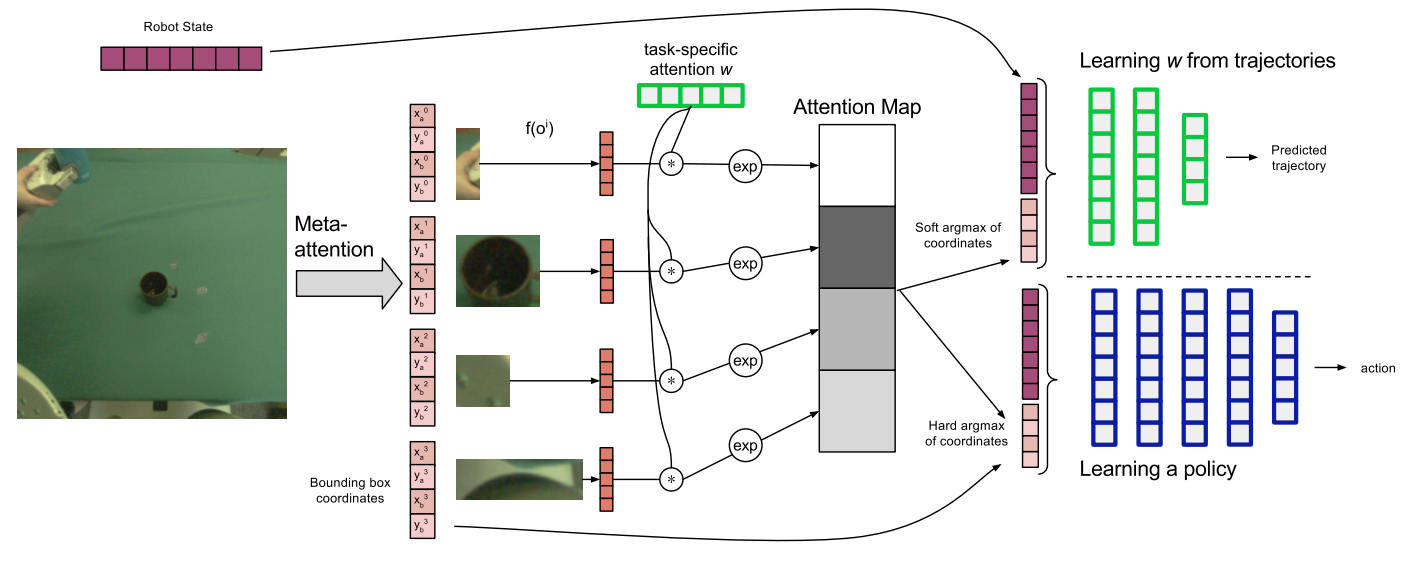
\includegraphics[width=0.8\textwidth]{figures/images/object_prior_framework.png}
    \caption{
            Robotic vision framework proposed in \cite{devin2018deep}. The framework is divided into different stages: \textbf{Meta-Attention}: Generates object proposals from an input image, trained on an object detection dataset, and shared across tasks; \textbf{Task-Specific Attention}: Focuses on relevant objects for a task using the meta-attention's semantic features; \textbf{Soft Attention}: Distributes attention as probabilities over object proposals using a Boltzmann distribution; \textbf{Movement Prediction Network}: Combines attended object information with the robot's state to predict the next action.
        }
    \label{fig:object_prior_framework}
\end{figure}
This preliminary work focused mainly on two tasks:
\begin{itemize}
    \item  \textit{Pouring Task}. The robot is required to pour contents from a bottle into a mug. The challenge is to locate the mug from an image without being explicitly provided its location, especially when different mugs are used during training and testing.
    \item \textit{Sweeping Task}. The robot must sweep an object (e.g., a plastic orange) into a dustpan, with both objects starting in different positions. This task requires the robot to adapt its approach based on the relative positions of the objects.
\end{itemize}
During testing, the authors focused on \textit{Category Generalization} and the ability to \textit{Ignore Distractor Objects}. For the former, the system was trained with only one type of mug and evaluated with other mugs (Figure \ref{fig:pouring_task_setting}). The results showed that the system successfully poured the contents into the correct mug, thanks to the learned task-specific attention weight that highlighted the mug features. For the latter, the authors designed a test where two mugs were present in the scene (Figure \ref{fig:task_specific_attention}). Since the model did not receive any conditioning signal indicating which mug to use, the authors fine-tuned the attention weight on trajectories where only the brown mug was used, demonstrating that this mechanism could focus on more specific features, such as the mug color.
\begin{figure}[t]
    \centering
    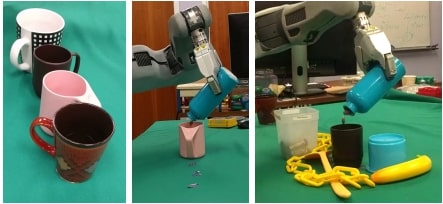
\includegraphics[width=0.6\textwidth]{figures/images/deep_object_centric_representation/pouring_task.jpg}
    \caption{Pouring task setting proposed in \cite{devin2018deep}. (Left) Mugs used for evaluation. Note that only the brown mug was seen during training. Center: Successful pouring into the pink mug. (Right) Pouring into the brown mug in a cluttered environment that was not seen during training.}
    \label{fig:pouring_task_setting}
\end{figure}

\begin{figure}[t]
    \centering
    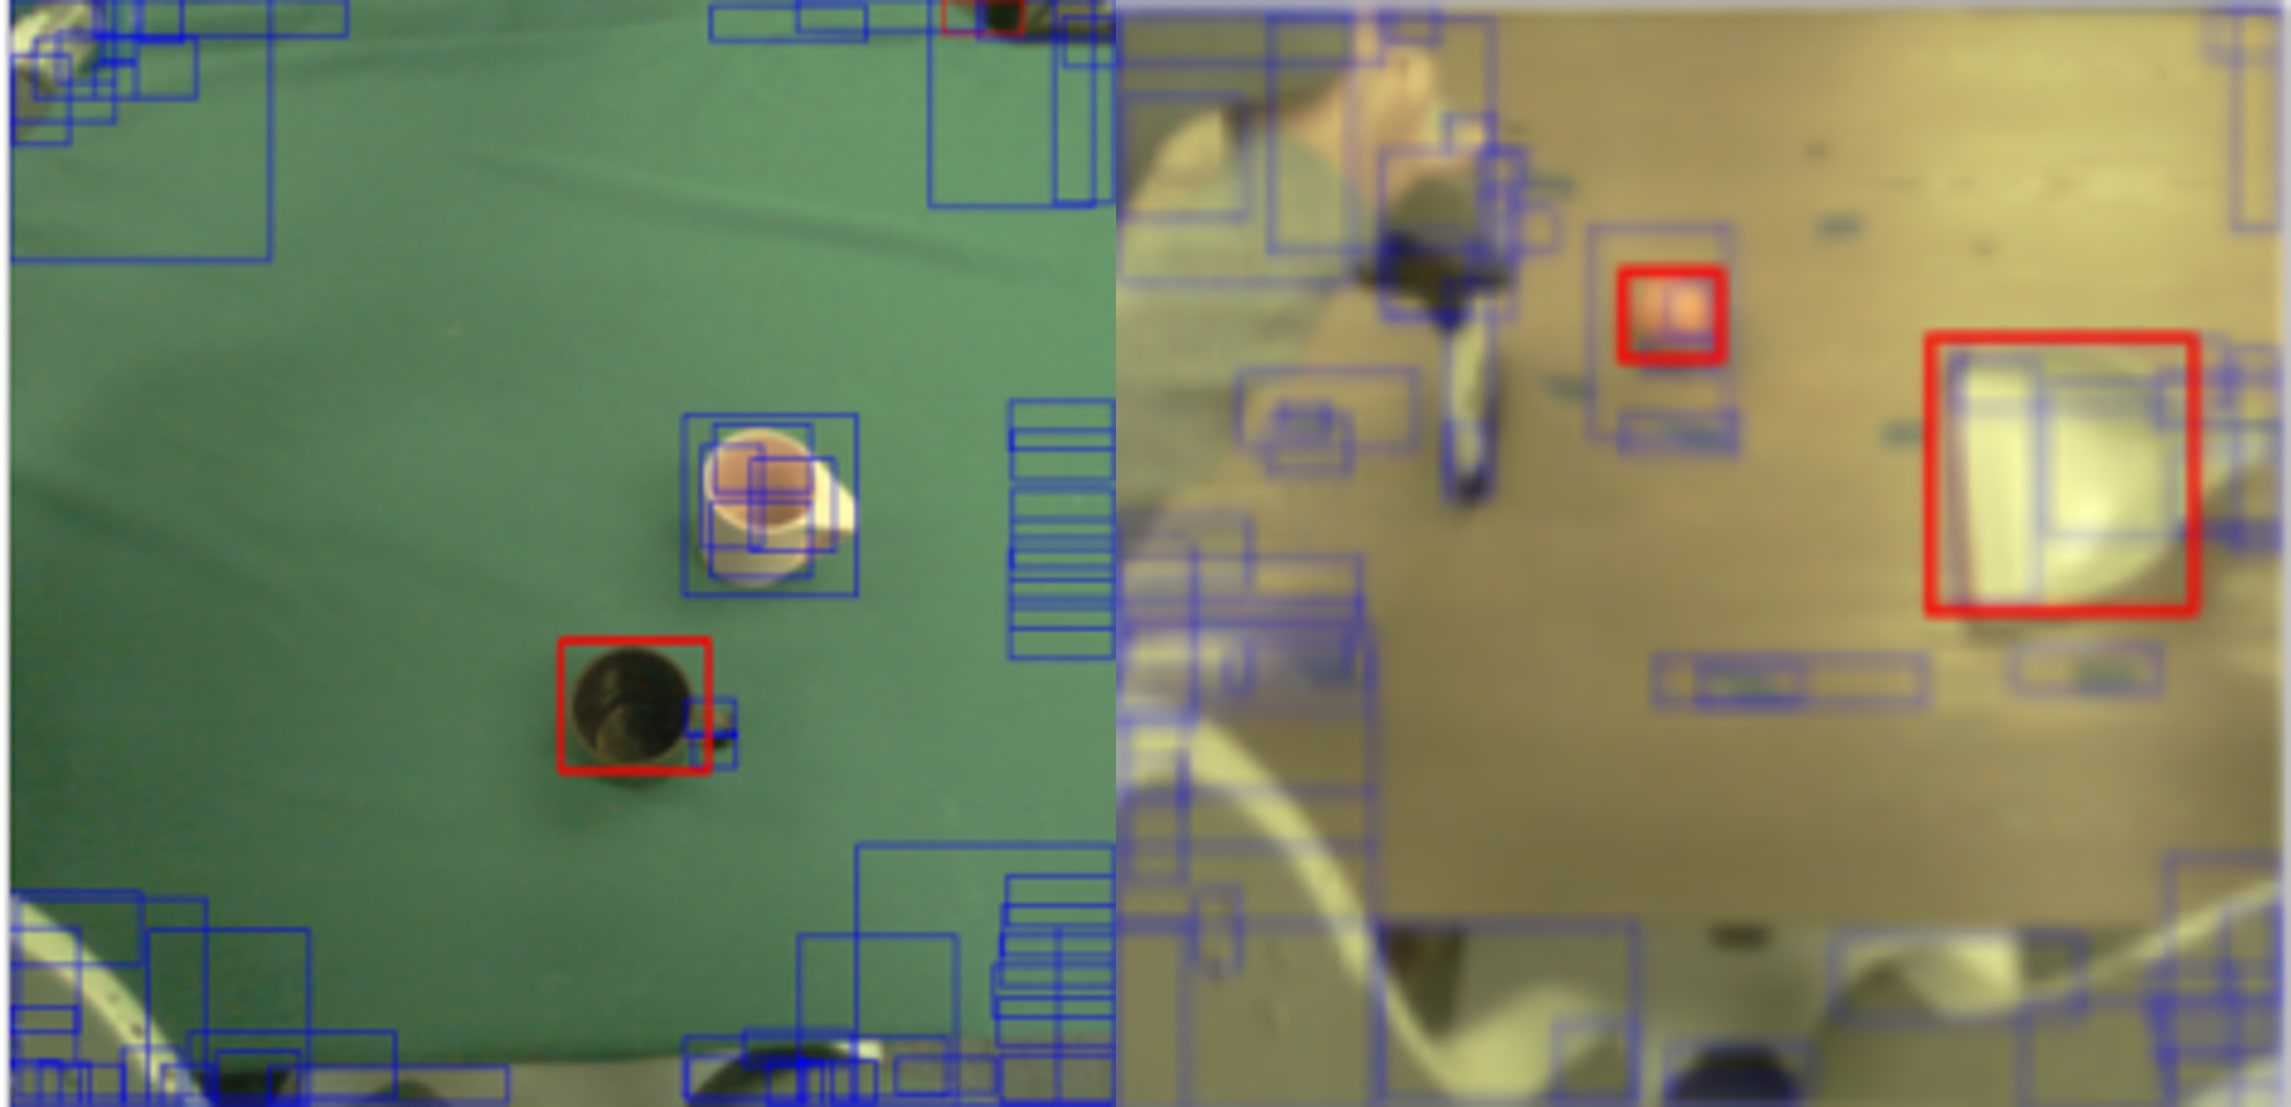
\includegraphics[width=0.6\textwidth]{figures/images/deep_object_centric_representation/mugs_distractors.jpg}
        \caption{The region proposals (meta-attention) are drawn in blue and the task-specific attended regions are drawn in red. For the Pouring task with distractor mug (pink) and target mug (brown), the attention locks on to the brown mug as its position defines the trajectory. For the sweeping task, two attention vectors are used, one attends to the orange and one attends to the dustpan.}
    \label{fig:task_specific_attention}
\end{figure}

In summary, this preliminary work demonstrated that leveraging object priors can facilitate category-level generalization by utilizing large, well-known datasets for the object-detection problem. However, the experimental setup was relatively simple, even in scenarios with distractor objects. The proposed system could handle distractor objects only after specific fine-tuning and was not able to dynamically discriminate between objects of interest and distractors based on task variations.

A recent work that follows a similar approach is proposed in \cite{zhu2023viola}. In this work, the authors introduced VIOLA (Visuomotor Imitation via Object-centric Learning) (Figure \ref{fig:viola_architecture}), an architecture inspired by the ideas presented in \cite{devin2018deep}. VIOLA uses an RPN and a ResNet18 \cite{resnet} to generate object proposals and produce a spatial feature map, respectively. It then constructs a \textit{per-step feature} vector, composed of three key elements: a \textbf{global context feature} that encodes the current task stage, an \textbf{eye-in-hand visual feature} to mitigate occlusion, and a \textbf{proprioceptive feature} that captures the robot state. These per-step features are concatenated to form a \textbf{history of observations}, which is designed to capture temporal dependencies and dynamic changes in object states. This tensor is then fed into a Transformer \cite{vaswani2017attention}, which leverages its intrinsic attention mechanism to automatically focus on the object of interest.
\begin{figure}[t]
    \centering
    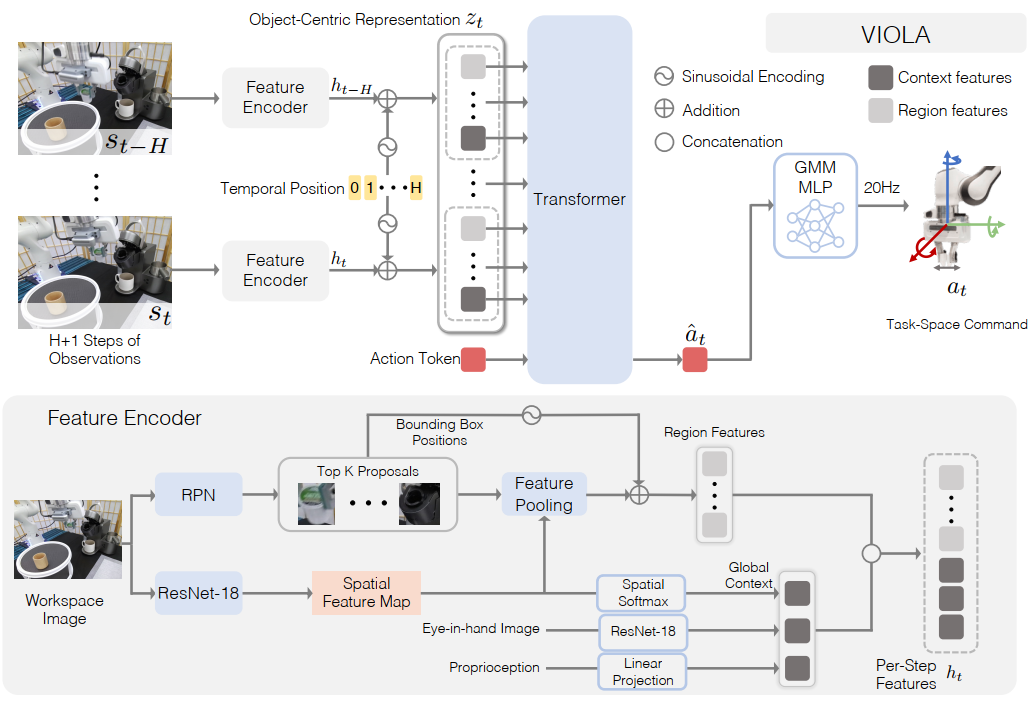
\includegraphics[width=0.7\textwidth]{figures/images/viola/viola_architecture.png}
        \caption{The VIOLA architecture proposed in \cite{zhu2023viola}. (Top) The overall control architecture is based on a Transformer module that processes a stack of \textit{per-step features} $h_{t}$, obtained from the Feature Encoder, to generate a final action embedding, which is then input into a GMM policy. (Bottom) The Feature Encoder builds both local and global features. Local features correspond to regions of interest extracted by the RPN. Global features are obtained by processing the workspace image, the image from the camera on the gripper, and proprioceptive information.
        }
    \label{fig:viola_architecture}
    
\end{figure}

\begin{figure}[t]
    \centering
    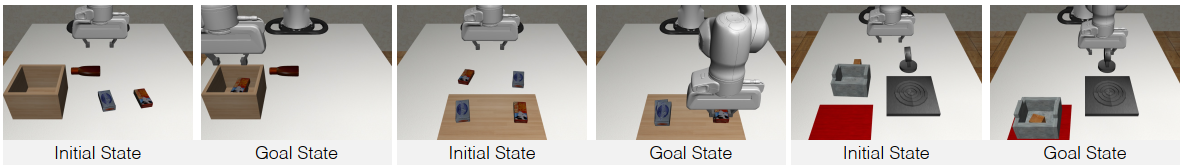
\includegraphics[width=0.9\textwidth]{figures/images/viola/viola_task.png}
    \caption{Simulation tasks on which the VIOLA \cite{zhu2023viola} method was tested. (Left) Sorting task. (Center) Stacking task. (Right) BUDS-Kitchen task}
    \label{fig:viola_task}
    
\end{figure}


This method was first evaluated in a simulation environment across three tasks, as depicted in Figure \ref{fig:viola_task}. Various testing scenarios were considered, including different object placements, the introduction of distractor objects, and changes in camera position. Generally speaking, VIOLA outperformed all baselines across these testing conditions, further demonstrating the utility of object priors in enhancing the robustness of such methods. However, similar to \cite{devin2018deep}, the testing scenarios were relatively simple, with clear distinctions between distractors and objects of interest. The distractors were objects never seen during the demonstration and were not involved in manipulation, making them relatively easy for the model to discriminate.

In the works discussed so far, the approach has primarily focused on leveraging object priors to directly predict the actions that the robot must perform. However, a different approach was proposed in \cite{belkhale2023plato}, where the authors introduced an alternative interpretation of object-centric concept. Instead of focusing on the robot perspective, they shifted the emphasis to the object perspective, proposing PLATO (Predicting Latent Affordances Through Object-Centric Play). PLATO is a learning framework that learns a \textbf{latent affordance space}, which describes how an object can be used (e.g., a block being grasped, a door knob being turned, or a drawer being opened).

The authors stated that learning affordances (i.e., object outcomes) from play, rather than plans (i.e., robot actions), enables simpler, more robust task representations that operate across varying time horizons. This approach improves policy effectiveness at test time by allowing the policy to reason more effectively about the environment. For example, given an affordance (e.g., a turned door knob) and a goal (e.g., an open door), the policy can infer the necessary behavior (e.g., reaching for the knob and rotating the gripper) to exploit that affordance.

To reach this objective authors started from the observation that a single-object manipulation is composed of the following three phases:
\begin{enumerate}
    \item \textbf{Pre-interaction}, when the robot prepares to interact with an object (e.g., reaching for a block).
    \item \textbf{Interaction}, when the robot and the object engage in joint actions (e.g., pushing or pulling the block).
    \item \textbf{Post-interaction}, when the robot separates from the object, and the object may come to rest (e.g., the block stops moving).
\end{enumerate}
Given these three phases, the algorithm learns a \textbf{latent affordance distribution}. Specifically, the architecture comprises three learnable modules:  $E$,  $E'$, and  $\pi$.  $E$ models the posterior distribution, mapping the full interaction trajectory  $\tau^{i}$ to the corresponding latent affordance distribution, from which the affordance embedding  $z$ is sampled.  $E'$ is the prior module used during rollout. It takes the current state and the goal state as input and generates the affordance embedding  $z'$. This module is trained to match the posterior distribution modeled by  $E$.  $\pi$ represents the current policy, which generates the action  $a^{i}$ given the current state  $s^{i}$, the desired goal  $o_g$, and the latent embedding  $z$.

These three modules are trained end-to-end by minimizing the loss function in Formula \ref{eq:plato_equation}, which includes three terms. The first two terms correspond to the policy  $\pi$, ensuring it matches the ground-truth trajectories in the interaction and pre-interaction phases. The last term is the KL-divergence, used to train the posterior and prior modules  $E$ and  $E'$.

\begin{equation}
    \label{eq:plato_equation}
    \begin{aligned}
        \mathcal{L}_{PLATO} = -\log \left(\pi\left(a_{1: H}^{(i)} \mid s_{1: H}^{(i)}, o_g, z\right)\right)- \\ 
        \alpha \log \left(\pi\left(a_{1: H}^{(-)} \mid s_{1: H}^{(-)}, o_g, z\right)\right)+ \\ 
        \beta \operatorname{KL}\left(p(z) \| p\left(z^{\prime}\right)\right)
    \end{aligned}
\end{equation}
\begin{figure}[t]
    \centering
    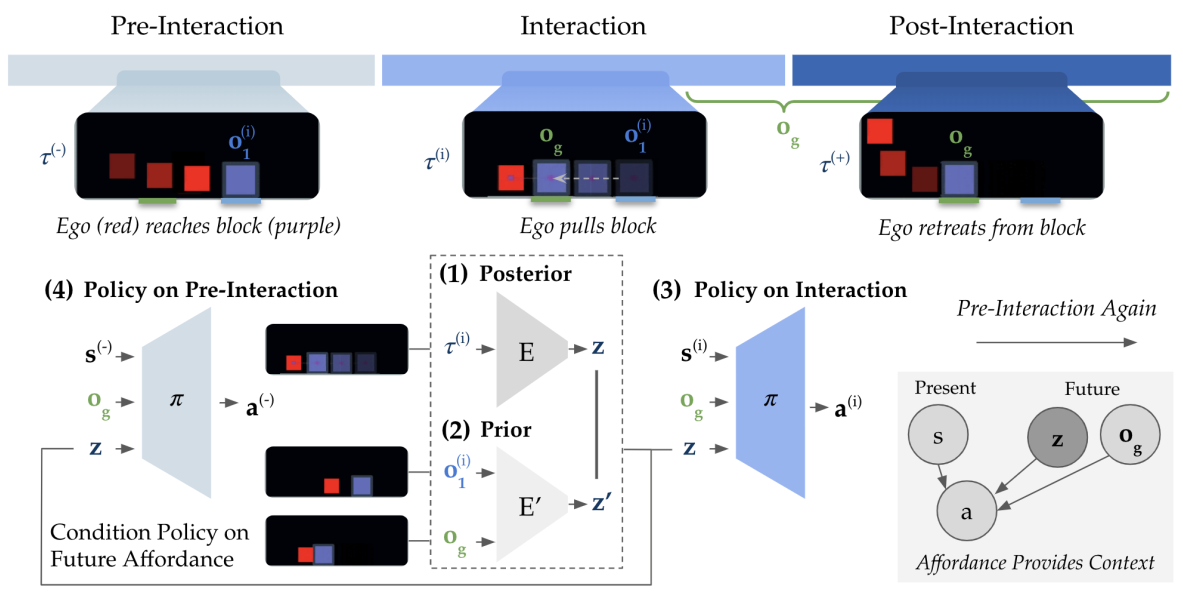
\includegraphics[width=0.7\textwidth]{figures/images/plato/plato.png}
    \caption{PLATO architecture proposed in \cite{belkhale2023plato}. The architecture is composed of different stages. (1) The posterior encoder \( E \) encodes the interaction sequence \( \tau^{(i)} \) into the affordance \( z \). (2) The prior encoder \( E' \) encodes the object initial state \( o^{(i)}_1 \) and goal state \( o_g \) to predict \( z \), with \( o_g \) sampled after the interaction. (3) The policy is trained to output actions during the interaction period conditioned on the affordance. Simultaneously, (4) it is trained to output actions during the pre-interaction period conditioned on the ``future" affordance.
    }
    \label{fig:plato}
    
\end{figure}

\begin{figure}[t]
    \centering
    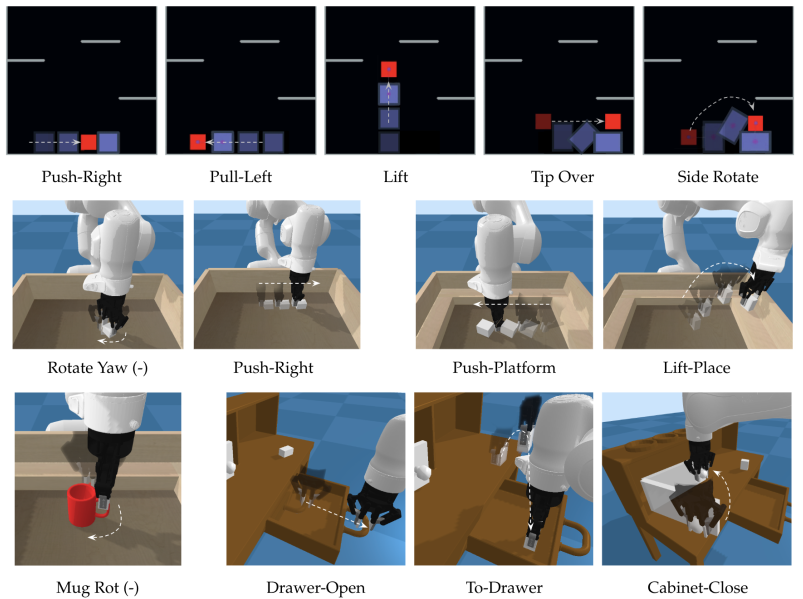
\includegraphics[width=0.7\textwidth]{figures/images/plato/tasks.png}
    \caption{ Testing scenarios and primitives proposed in \cite{belkhale2023plato}. (Top) \textbf{Block2D} Environment primitive examples. (Center) \textbf{Block3D} and \textbf{Block3DPlatform} primitive examples. (Bottom) The left image shows an example primitive in \textbf{Mug3D-Platforms}. The right three images show sample tasks from \textbf{Playroom3D}.}
    \label{fig:plato_task}
    
\end{figure}

Finally, this method was tested in a variety of scenarios, including both single-object and multiple-object manipulation with different manipulation primitives (Figure \ref{fig:plato_task}). However, in the multi-object scenarios, the system was only tested on single-object manipulation primitives.

This work is particularly noteworthy as it demonstrates that a policy can be learned by solving an inverse problem, starting from object affordances and deriving the corresponding robot trajectories. It also shows that the policy can be conditioned based on the desired goal state. However, certain aspects were not addressed in this work, such as the potential presence of distractor objects and tasks requiring the manipulation of multiple objects. Additionally, the affordances were learned in the object space (i.e., with known object poses) rather than in the high-level image space.

The works discussed in this paragraph highlight the significant research efforts aimed at modeling the manipulation problem from an object-centric perspective. These efforts either focus on the affordances of the object (i.e., the possible movements the object allows) or introduce object priors defined by regions of interest that may contain the object to be manipulated, with results demonstrated in both simulated and real-world environments. However, the methods presented so far primarily address single-task scenarios, where distractor objects can be easily identified as they remain constant across demonstrations. In contrast, this thesis proposes a solution for a more challenging scenario in which the robot operates in a multi-variation environment. This environment includes multiple similar objects, which may serve as either targets or distractors depending on the specific task variation.
